% Results from campaign_su_mu_20260802-134343/mu_tdllow (qat_only + qat_pruned)
% and campaign_su_mu_20260809-080711/mu_tdllow (qat_activation / W*A8).
% Numbers: log-linear interpolation of BLER curves at targets 10% and 1%.
%
% Figure assets:
%   campaign_su_mu_20260809-080711/figures/mu_tdllow/bler_qat_activation.pdf
%   campaign_su_mu_20260802-134343/figures/mu_tdllow/bler_qat_pruned.pdf
%   insight_fp4_sparsity/figures/weight_histogram_zoom.pdf
%   insight_fp4_sparsity/figures/sparsity_bars.pdf

\section{Experimental Results and Discussion}
\label{sec:results}

\begin{table}[t]
\centering
\caption{System, training, and evaluation parameters.}
\label{tab:sim_params}
\footnotesize
\setlength{\tabcolsep}{3pt}
\begin{tabular}{@{}p{0.44\columnwidth}p{0.50\columnwidth}@{}}
\toprule
Parameter & Value \\
\midrule
Users $\times$ layers (eval) & $2\times1$ \\
Receive antennas $N_{\mathrm{rx}}$ & 4 \\
Carrier / SCS & 2.14\,GHz / 30\,kHz \\
OFDM symbols & 14 \\
PRBs (train / eval) & 4 / 132 \\
MCS / code rate $R$ (Table~1 \cite{3gpp38214})
  & index 14 / $R\approx0.48$ (16-QAM) \\
DMRS & type~1, mapping~A, +1 position \\
Channel (train) & 3GPP UMi, speeds $[0,56]$\,m/s \\
Channel (eval) & UE1 TDL-B100/400 ($100$\,ns, $400$\,Hz) \cite{scamnrx} \\
 & UE2 TDL-C300/100 ($300$\,ns, $100$\,Hz) \\
NRX depth $N_{\mathrm{it}}$ / state width $d_s$ & 8 / 56 \\
Batch size $N_B$ & 128 \\
FP8/FP4/INT8/INT4 QAT & $5{\times}10^{4}$ at $10^{-4}$; then $2{\times}10^{5}$ at $5{\times}10^{-5}$ \\
%INT8/INT4 QAT & $10^{6}$; then $9{\times}10^{6}$ steps, both at $10^{-4}$ \\
W$b$A8 fine-tune & $5{\times}10^{4}$ at $10^{-4}$; then $10^{5}$ at $5{\times}10^{-5}$ \\
Prune recovery & $5{\times}10^{3}$ at $5{\times}10^{-5}$; then $10^{4}$ at $2{\times}10^{-5}$ \\
\bottomrule
\end{tabular}\\[2pt]
{\scriptsize Optimizer rows report the step count and learning rate for two successive Adam phases.}
\end{table}

\begin{comment}

\begin{figure*}[t]
    \centering
    \begin{subfigure}[t]{0.48\linewidth}
        \centering
        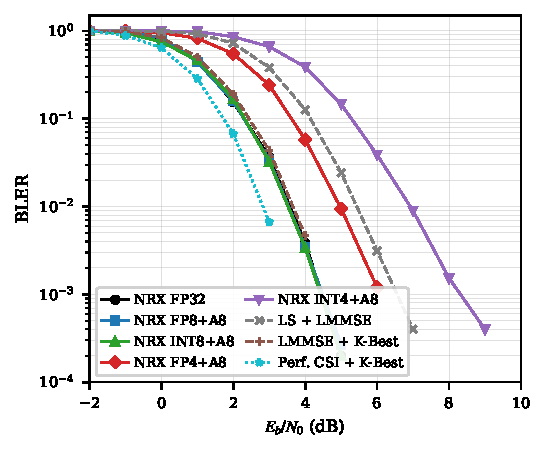
\includegraphics[width=\linewidth]{campaign_su_mu_20260809-080711/figures/mu_tdllow/bler_qat_activation.pdf}
        \caption{Weight+A8 QAT (MU-MIMO, TDL-B/C, $U{=}2$, 16-QAM)}
        \label{fig:bler_qat}
    \end{subfigure}\hfill
    \begin{subfigure}[t]{0.48\linewidth}
        \centering
        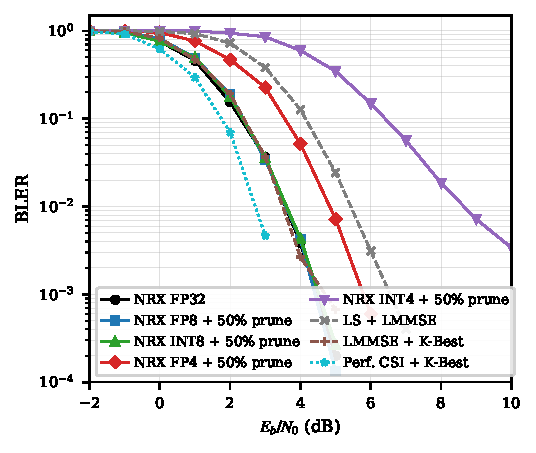
\includegraphics[width=\linewidth]{campaign_su_mu_20260802-134343/figures/mu_tdllow/bler_qat_pruned.pdf}
        \caption{Weight QAT + 50\% magnitude pruning}
        \label{fig:bler_prune}
    \end{subfigure}
    \caption{BLER vs.\ $E_b/N_0$ for the neural receiver on
    TDL-B100/400 (UE1) and TDL-C300/100 (UE2).
    Both panels share the same axes and baseline curves (FP32, LS--\gls{LMMSE},
    \gls{LMMSE}--K-Best, perfect-CSI K-Best). Panel~(a) shows joint weight and
    INT8 asymmetric post-\gls{ReLU} activation \gls{QAT} (W$b$A8) in
    FP8~(E4M3), INT8, FP4~(E2M1), and INT4; panel~(b) shows the same
    weight-QAT checkpoints after 50\% global magnitude pruning of
    pointwise and dense kernels.}
    \label{fig:BLER}
\end{figure*}
\end{comment}
\begin{figure*}[t]
    \centering
    \begin{subfigure}[t]{0.48\linewidth}
        \centering
        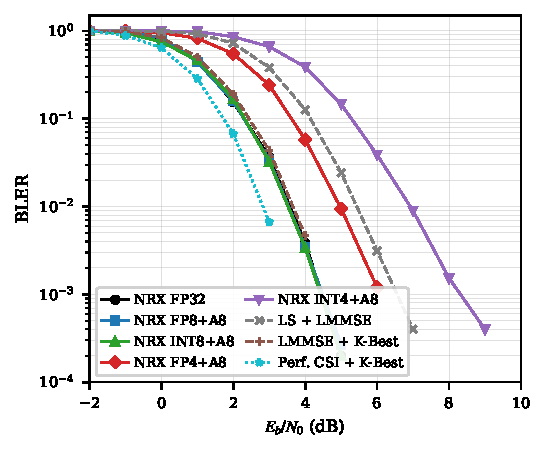
\includegraphics[width=\linewidth]{campaign_su_mu_20260809-080711/figures/mu_tdllow/bler_qat_activation.pdf}
        \caption{W$b$A8 QAT}
        \label{fig:bler_qat}
    \end{subfigure}\hfill
    \begin{subfigure}[t]{0.48\linewidth}
        \centering
        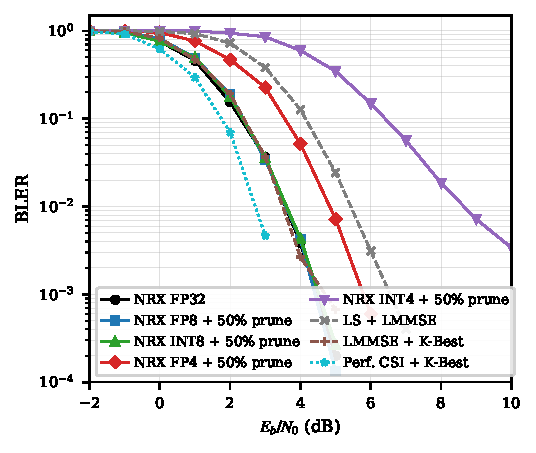
\includegraphics[width=\linewidth]{campaign_su_mu_20260802-134343/figures/mu_tdllow/bler_qat_pruned.pdf}
        \caption{Weight QAT + 50\% pruning}
        \label{fig:bler_prune}
    \end{subfigure}
    \caption{\gls{BLER} versus $E_b/N_0$ on TDL-B100/400 \& TDL-C300/100 for
    (a) W$b$A8 \gls{QAT}, where $b\in\{4,8\}$ denotes the weight bit
    width, and (b) 50\%-pruned weight-\gls{QAT} checkpoints.}
    \label{fig:BLER}
\end{figure*}

\begin{figure*}[t]
    \centering
    \begin{subfigure}[t]{0.40\linewidth}
        \centering
        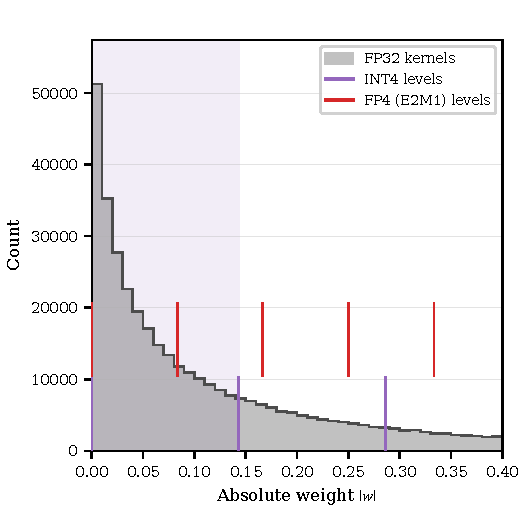
\includegraphics[width=\linewidth]{insight_fp4_sparsity/figures/weight_histogram_zoom.pdf}
        \caption{Normalized weight histogram.}
        \label{fig:weight_hist}
    \end{subfigure}\hfill
    \begin{subfigure}[t]{0.43\linewidth}
        \centering
        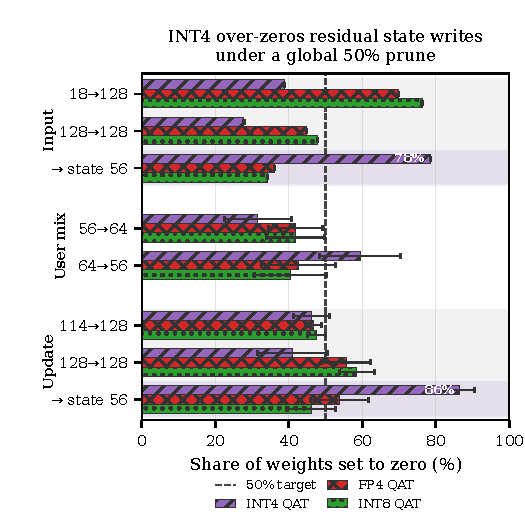
\includegraphics[width=\linewidth]{insight_fp4_sparsity/figures/sparsity_bars.pdf}
        \caption{Per-kernel sparsity after global $50\%$ pruning.}
        \label{fig:sparsity_layers}
    \end{subfigure}
    \caption{FP4 robustness diagnostics. Panel~(a) compares
    per-channel abs-max-normalized \texttt{FP32} weight magnitudes
    with the INT4 and FP4 grids. Panel~(b) groups kernel sparsity by
    receiver stage after global $50\%$ pruning. Its y-axis labels
    give $C_{\mathrm{in}}{\to}C_{\mathrm{out}}$. Labels ending in
    ``state 56'' denote residual state writes. Error bars show the
    standard deviation across eight unrolled blocks. The Input CNN has
    one instance.}
    \label{fig:fp4_diagnostics}
\end{figure*}

\begin{table}[t]
    \centering
    \caption{Weight-only QAT vs.\ W+A8 on DoubleTDL-low, interpolated from
    the same paired eval. W is the weight-QAT checkpoint; W+A8 is
    quantization-aware fine-tuning of that checkpoint with INT8 asymmetric
    post-\gls{ReLU} activations Table~\ref{tab:sim_params}.
    $\Delta$ is $E_b/N_0$ of W+A8 minus W.}
    \label{tab:wo_vs_a8}
    \begin{tabular}{lcccc}
    \toprule
     & \multicolumn{2}{c}{$E_b/N_0$ @ $10\%$ (dB)} & \multicolumn{2}{c}{$\Delta$ A8$-$W (dB)} \\
    \cmidrule(lr){2-3}\cmidrule(lr){4-5}
    Format & W-only & W+A8 & $10\%$ & $1\%$ \\
    \midrule
    FP8 (E4M3) & 2.29 & 2.30 & +0.00 & +0.01 \\
    INT8 & 2.24 & 2.31 & +0.08 & +0.01 \\
    FP4 (E2M1) & 3.62 & 3.62 & +0.00 & $-0.01$ \\
    INT4$^{\ddagger}$ & 5.60 & 5.29 & $-0.32$ & $-0.33$ \\
    \bottomrule
    \end{tabular}\\[2pt]
    \footnotesize{$^{\ddagger}$For INT4, negative $\Delta$ reflects quantization-aware fine-tuning of the weight-only parent, not a benefit from activation quantization.}
    \end{table}
    
\begin{table}[t]
\centering
\caption{Analytic complexity per 5G~NR slot (132~PRB, 2~users,
8 iterations). Weights include biases, scales, and a sparse bitmask.}
\label{tab:complexity}
\footnotesize
\setlength{\tabcolsep}{3.5pt}
\begin{tabular}{@{}lccccc@{}}
\toprule
Config. & W/A & Spars. & Wt.\ (KiB)  & BOPs (T) \\
\midrule
FP32        & 32/32 & --   & 1708.5  & 19.7 \\
FP16        & 16/16 & --   &  862.1  &  4.9 \\
W8A8        & 8/8   & --   &  453.1  &  1.2 \\
W8A8+P      & 8/8   & 50\% &  310.9 &  0.7 \\
W4A8        & 4/8   & --   &  241.6   0.6 \\
W4A8+P      & 4/8   & 50\% &  194.1   0.3 \\
\bottomrule
\end{tabular}
\end{table}



\begin{comment}
\toprule
Config. & W/A & Spars. & Wt.\ (KiB) & MACs (G) & BOPs (T) \\
\midrule
FP32        & 32/32 & --   & 1708.5 & 19.22 & 19.7 \\
FP16        & 16/16 & --   &  862.1 & 19.22 &  4.9 \\
W8A8        & 8/8   & --   &  453.1 & 19.22 &  1.2 \\
W8A8+P      & 8/8   & 50\% &  310.9 & 10.61 &  0.7 \\
W4A8        & 4/8   & --   &  241.6 & 19.22 &  0.6 \\
W4A8+P      & 4/8   & 50\% &  194.1 & 10.61 &  0.3 \\
\bottomrule
\end{comment}

We evaluate weight \gls{QAT} with FP8~(E4M3), INT8, FP4~(E2M1), and
INT4. From each weight-only checkpoint, we separately derive a W$b$A8
model and a 50\%-pruned model. Experiments use the 3GPP-compliant
two-user PUSCH setup and optimizer budgets in
Table~\ref{tab:sim_params}.\footnote{Model weights and experiment scripts will be released at \url{https://github.com/saiksaketh/quantized_neural_rx/tree/feature/nrx-qat} upon acceptance to a possible IEEE conference venue.}
We report \gls{BLER} versus rate-adjusted $E_b/N_0$ at $10\%$ and
$1\%$ targets. Baselines include the full-precision (\texttt{FP32}) neural receiver,
LS channel estimation with \gls{LMMSE} equalization, \gls{LMMSE} channel
estimation with K-Best detection, and ideal K-Best detection with
perfect CSI (Fig.~\ref{fig:BLER}). An analytic model estimates storage
and bit-operations on the evaluation graph.

\vspace{-2mm}

\subsection{Activation Quantization is Radio-Neutral on Link Performance at 8~Bits}
\label{sec:res_a8}
Figure~\ref{fig:bler_qat} shows \gls{BLER} for the unpruned QAT
receivers with joint weight and activation quantization.
Table~\ref{tab:wo_vs_a8} reports the corresponding weight-only
operating points. FP8~(E4M3) and INT8 W$b$A8 receivers remain within
$0.05$\,dB of \texttt{FP32} at $10\%$ and $1\%$ \gls{BLER}. Adding A8
to the weight-only checkpoints changes the required $E_b/N_0$ by at
most $0.08$\,dB at either target. Both receivers outperform LS--\gls{LMMSE}
by approximately $1.83$--$1.91$\,dB and remain within
$\sim0.2$\,dB of \gls{LMMSE}--K-Best.\footnote{LS--\gls{LMMSE} and \gls{LMMSE}--K-Best use
floating-point arithmetic. Fixed-point arithmetic may increase
\gls{BLER} due to additional quantization error.} Thus, A8 causes no observed link
penalty in this setting. Section~\ref{sec:res_prune} evaluates pruning
from weight-only checkpoints.

\vspace{-2mm}

\subsection{FP4 Halves the 4-bit Loss}
\label{sec:res_fp4}
For weight-only QAT, the format strongly affects 4-bit performance
(Table~\ref{tab:wo_vs_a8}). At $10\%$ and $1\%$ \gls{BLER}, FP4~(E2M1)
needs $1.32$\,dB and $1.40$\,dB more $E_b/N_0$ than \texttt{FP32}
and beats LS--\gls{LMMSE} by about $0.5$\,dB. INT4 needs $3.3$--$3.7$\,dB
more than \texttt{FP32}. That gap is $1.98$\,dB and $2.27$\,dB larger
than FP4's, and INT4 also trails LS--\gls{LMMSE}. The nonuniform
E2M1 grid therefore more than halves the 4-bit SNR penalty at both
targets. Activation quantization retains FP4's advantage (Fig.~\ref{fig:bler_qat}).

We apply the per-channel abs-max normalization in
\eqref{eq:absmax_scale} to the $0.404$\,M trained \texttt{FP32}
prune-eligible pointwise and dense weights
(Fig.~\ref{fig:weight_hist}). For a normalized weight $w$, $65\%$ of
values satisfy $|w|<1/7\approx0.14$, the first nonzero INT4 magnitude.
FP4 adds a level at $1/12\approx0.08$. Moreover, $79\%$ of the weights
satisfy $|w|<0.25$. Over $[0,0.25]$, INT4 provides two magnitudes,
including zero, whereas FP4 provides four magnitudes
($0$, $0.08$, $0.17$, and $0.25$). The denser E2M1 grid better
resolves the distribution body and provides reconstruction levels
unavailable under uniform INT4.

\vspace{-2mm}

\subsection{Post-QAT Magnitude Pruning}
\label{sec:res_prune}
Figure~\ref{fig:bler_prune} shows weight-only checkpoints after 50\%
global pruning of eligible kernels. Depthwise and readout layers
remain dense. Penalties use each format's unpruned
weight-only parent, not panel~(a). At 8~bits, pruning changes the
required $E_b/N_0$ by at most $0.13$\,dB at either target. FP4 changes
by $-0.07$/$-0.10$\,dB after pruning and remains ahead of LS--\gls{LMMSE}.
In contrast, pruning adds $0.95$--$1.29$\,dB to INT4, which trails
LS--\gls{LMMSE} by more than $2$\,dB. \emph{Thus, FP4 tolerates 50\% pruning
with negligible radio impact, whereas INT4 with pruning degrades sharply.}

Figure~\ref{fig:sparsity_layers} reports the fraction of weights
zeroed in each labeled kernel. The global 50\% target applies over all
eligible coefficients, not per kernel. Under INT4, residual
update-to-state kernels average $86.5\%$ zeros (maximum $91.4\%$),
compared with $53.8\%$ (maximum $66.2\%$) under FP4. The Input CNN
state-write kernel reaches $78.5\%$ and $36.1\%$, respectively. Thus,
INT4 concentrates pruning in residual paths, while FP4 sparsity
remains comparable to INT8. Together with the denser near-zero FP4
grid in Fig.~\ref{fig:weight_hist}, this pattern is consistent with
FP4's higher pruning robustness.

Relative to \texttt{FP32}, the modeled W4A8+P configuration yields
$66\times$ and $8.8\times$ reductions in \glspl{BOP} and weight
footprint, respectively. W8A8 and W4A8 reduce \glspl{BOP} by
$16\times$ and $33\times$, respectively, and reduce stored weight
footprints by $3.8\times$ and $7.1\times$. The radio experiments
evaluate W$b$A8 and pruning separately, whereas the +P rows project
their combined analytic cost. Table~\ref{tab:complexity} reports
analytic costs on the evaluation graph with 132~\glspl{PRB}, 2~users,
and 8 iterations. Each slot requires $19.22$\,G multiply--accumulate
operations (MACs). Of these, $76\%$ arise from $1{\times}1$ pointwise
convolutions, the dominant GEMM-like kernels targeted by low-bit
quantization. We estimate \glspl{BOP} as
\[
  \mathrm{BOPs}
  = \sum_{\ell}\mathrm{MAC}_{\ell}\,b_{w,\ell}b_{a,\ell},
\]
where $b_{w,\ell}$ and $b_{a,\ell}$ are the weight and activation
widths of layer $\ell$. For eligible pruned kernels,
$\mathrm{MAC}_{\ell}$ is scaled by the retained-weight fraction.